\documentclass{beamer}

%
% Common preamble for all three parts.
%
\usepackage[T1]{fontenc}
\usepackage[utf8]{inputenc}
\usepackage[catalan]{babel}
\usepackage{amsmath}
\usepackage{color}
\usepackage{minted}
\usepackage{hyperref}
\usepackage{multicol}
\usepackage{tabularx, booktabs}
\usepackage{tikz}

% only inline todonotes work
\usepackage{xkeyval}
\usepackage[textsize=small]{todonotes}
\presetkeys{todonotes}{inline}{}

\usetikzlibrary{shapes,arrows,positioning,shadows}

% no nav buttons
\usenavigationsymbolstemplate{}

\newcommand{\bftt}[1]{\textbf{\texttt{#1}}}
\newcommand{\comment}[1]{{\color[HTML]{008080}\textit{\textbf{\texttt{#1}}}}}
\newcommand{\cmd}[1]{{\color[HTML]{008000}\bftt{#1}}}
\newcommand{\bs}{\char`\\}
\newcommand{\cmdbs}[1]{\cmd{\bs#1}}
\newcommand{\lcb}{\char '173}
\newcommand{\rcb}{\char '175}
\newcommand{\cmdbegin}[1]{\cmdbs{begin\lcb}\bftt{#1}\cmd{\rcb}}
\newcommand{\cmdend}[1]{\cmdbs{end\lcb}\bftt{#1}\cmd{\rcb}}

\newcommand{\wllogo}{\textbf{Overleaf}}

% this is where the example source files are loaded from
% do not include a trailing slash
\newcommand{\fileuri}{https://raw.github.com/pastells/curs-latex/master/ca}

\newcommand{\wlserver}{https://www.overleaf.com}
\newcommand{\wlnewdoc}[1]{\wlserver/docs?snip\_uri=\fileuri/#1\&splash=none}

\def\tikzname{Ti\emph{k}Z}

% from http://tex.stackexchange.com/questions/5226/keyboard-font-for-latex
\newcommand*\keystroke[1]{%
  \tikz[baseline=(key.base)]
    \node[%
      draw,
      fill=white,
      drop shadow={shadow xshift=0.25ex,shadow yshift=-0.25ex,fill=black,opacity=0.75},
      rectangle,
      rounded corners=2pt,
      inner sep=1pt,
      line width=0.5pt,
      font=\scriptsize\sffamily
    ](key) {#1\strut}
  ;
}
\newcommand{\keystrokebftt}[1]{\keystroke{\bftt{#1}}}

% stolen from minted.dtx
\newenvironment{exampletwoup}
  {\VerbatimEnvironment
   \begin{VerbatimOut}{example.out}}
  {\end{VerbatimOut}
   \setlength{\parindent}{0pt}
   \fbox{\begin{tabular}{l|l}
   \begin{minipage}{0.55\linewidth}
     \inputminted[fontsize=\small,resetmargins]{latex}{example.out}
   \end{minipage} &
   \begin{minipage}{0.35\linewidth}
     \input{example.out}
   \end{minipage}
   \end{tabular}}}

\newenvironment{exampletwouptiny}
  {\VerbatimEnvironment
   \begin{VerbatimOut}{example.out}}
  {\end{VerbatimOut}
   \setlength{\parindent}{0pt}
   \fbox{\begin{tabular}{l|l}
   \begin{minipage}{0.55\linewidth}
     \inputminted[fontsize=\scriptsize,resetmargins]{latex}{example.out}
   \end{minipage} &
   \begin{minipage}{0.35\linewidth}
     \setlength{\parskip}{6pt plus 1pt minus 1pt}%
     \raggedright\scriptsize\input{example.out}
   \end{minipage}
   \end{tabular}}}

\newenvironment{exampletwouptinynoframe}
  {\VerbatimEnvironment
   \begin{VerbatimOut}{example.out}}
  {\end{VerbatimOut}
   \setlength{\parindent}{0pt}
   \begin{tabular}{l|l}
   \begin{minipage}{0.55\linewidth}
     \inputminted[fontsize=\scriptsize,resetmargins]{latex}{example.out}
   \end{minipage} &
   \begin{minipage}{0.35\linewidth}
     \setlength{\parskip}{6pt plus 1pt minus 1pt}%
     \raggedright\scriptsize\input{example.out}
   \end{minipage}
   \end{tabular}}

\title{Introducció Interactiva a \LaTeX}
\author{Pol Pastells}
\titlegraphic{%

\includegraphics[height=24pt]{overleaf} \quad

\includegraphics[height=24pt]{logo_UB.png}
}


\subtitle{Part 3: Presentacions i altres}

\newcommand{\mar}[1]{\todo[color=green!40]{#1}}
\newcommand{\andreu}[1]{\todo[color=purple!40]{#1}}

\begin{document}

%%%%%%%%%%%%%%%%%%%%%%%%%%%%%%%%%%%%%%%%%%%%%%%%%%%%%%%%%%%%%%%%%%%%%%%%%%%%%%%
%%%%%%%%%%%%%%%%%%%%%%%%%%%%%%%%%%%%%%%%%%%%%%%%%%%%%%%%%%%%%%%%%%%%%%%%%%%%%%%
%%%%%%%%%%%%%%%%%%%%%%%%%%%%%%%%%%%%%%%%%%%%%%%%%%%%%%%%%%%%%%%%%%%%%%%%%%%%%%%
\begin{frame}
\titlepage
\end{frame}

%%%%%%%%%%%%%%%%%%%%%%%%%%%%%%%%%%%%%%%%%%%%%%%%%%%%%%%%%%%%%%%%%%%%%%%%%%%%%%%
%%%%%%%%%%%%%%%%%%%%%%%%%%%%%%%%%%%%%%%%%%%%%%%%%%%%%%%%%%%%%%%%%%%%%%%%%%%%%%%
%%%%%%%%%%%%%%%%%%%%%%%%%%%%%%%%%%%%%%%%%%%%%%%%%%%%%%%%%%%%%%%%%%%%%%%%%%%%%%%
%\begin{frame}{Setup}
%\begin{itemize}
%\item Go to this URL in Google Chrome (\emph{not} Internet Explorer) to open
%these slides on your computer:
%\vskip 2em
%\begin{center}
%\fbox{\url{http://bit.ly/12WWWqj}}
%\end{center}
%\vskip 2em
%\item Here are the slides from the previous tutorial, for reference:
%\begin{center}
%\vskip 1em
%\fbox{\href{https://dl.dropboxusercontent.com/u/31383671/site/latex_course_v2/part1.pdf}{Part 1: The Basics}}
%\vskip 1em
%\fbox{\href{https://dl.dropboxusercontent.com/u/31383671/site/latex_course_v2/part2.pdf}{Part 2: Structured Documents \& More}}
%\end{center}
%\end{itemize}
%\end{frame}

%%%%%%%%%%%%%%%%%%%%%%%%%%%%%%%%%%%%%%%%%%%%%%%%%%%%%%%%%%%%%%%%%%%%%%%%%%%%%%%
%%%%%%%%%%%%%%%%%%%%%%%%%%%%%%%%%%%%%%%%%%%%%%%%%%%%%%%%%%%%%%%%%%%%%%%%%%%%%%%
%%%%%%%%%%%%%%%%%%%%%%%%%%%%%%%%%%%%%%%%%%%%%%%%%%%%%%%%%%%%%%%%%%%%%%%%%%%%%%%
\section{\LaTeX{} Recap}

%%%%%%%%%%%%%%%%%%%%%%%%%%%%%%%%%%%%%%%%%%%%%%%%%%%%%%%%%%%%%%%%%%%%%%%%%%%%%%%
%%%%%%%%%%%%%%%%%%%%%%%%%%%%%%%%%%%%%%%%%%%%%%%%%%%%%%%%%%%%%%%%%%%%%%%%%%%%%%%
%%%%%%%%%%%%%%%%%%%%%%%%%%%%%%%%%%%%%%%%%%%%%%%%%%%%%%%%%%%%%%%%%%%%%%%%%%%%%%%
\begin{frame}[fragile]{\insertsection}
\begin{itemize}
\item You write your document in \texttt{plain text} with \cmd{ordres} that
describe its structure i meaning.
\item The \texttt{latex} program processes your text i ordres to produce a
beautifully formatted document.
\end{itemize}
\vskip 2ex
\begin{center}
\begin{minted}[frame=single]{latex}
The rain in Spain falls \emph{mainly} on the plain.
\end{minted}
\vskip 2ex
\tikz\node[single arrow,fill=gray,font=\ttfamily\bfseries,%
  rotate=270,xshift=-1em]{latex};
\vskip 2ex
\fbox{The rain in Spain falls \emph{mainly} on the plain.}
\end{center}
\end{frame}

%%%%%%%%%%%%%%%%%%%%%%%%%%%%%%%%%%%%%%%%%%%%%%%%%%%%%%%%%%%%%%%%%%%%%%%%%%%%%%%
%%%%%%%%%%%%%%%%%%%%%%%%%%%%%%%%%%%%%%%%%%%%%%%%%%%%%%%%%%%%%%%%%%%%%%%%%%%%%%%
%%%%%%%%%%%%%%%%%%%%%%%%%%%%%%%%%%%%%%%%%%%%%%%%%%%%%%%%%%%%%%%%%%%%%%%%%%%%%%%
\begin{frame}[fragile]{\insertsection: ordres \& Arguments}
\begin{itemize}
\item A ordre starts with a \emph{backslash} \keystrokebftt{\bs}.
\item Some ordres take an \emph{argument} in curly braces \keystrokebftt{\{}
\keystrokebftt{\}}.
\item Some ordres also take \emph{optional arguments} in square brackets \keystrokebftt{[} \keystrokebftt{]}.
\vskip 2ex
\begin{exampletwouptiny}

\includegraphics[
  width=0.5\textwidth]{gerbil}


\includegraphics[
  width=0.3\textwidth,
  angle=270]{gerbil}
\end{exampletwouptiny}
\end{itemize}

\tiny{Image license: \href{https://pixabay.com/en/animal-apple-attractive-beautiful-1239390/}{CC0}}
\end{frame}

%%%%%%%%%%%%%%%%%%%%%%%%%%%%%%%%%%%%%%%%%%%%%%%%%%%%%%%%%%%%%%%%%%%%%%%%%%%%%%%
%%%%%%%%%%%%%%%%%%%%%%%%%%%%%%%%%%%%%%%%%%%%%%%%%%%%%%%%%%%%%%%%%%%%%%%%%%%%%%%
%%%%%%%%%%%%%%%%%%%%%%%%%%%%%%%%%%%%%%%%%%%%%%%%%%%%%%%%%%%%%%%%%%%%%%%%%%%%%%%
\begin{frame}[fragile]{\insertsection: Environments}
\begin{itemize}
\item The \cmdbs{begin} i \cmdbs{end} ordres are used to create many
different environments --- contexts.

\item The \bftt{itemize} i \bftt{enumerate} environments make lists.
\vskip 2ex
\begin{exampletwouptiny}
\begin{itemize} % for bullet points
\item Biscuits
\item Tea
\end{itemize}

\begin{enumerate} % for numbers
\item Biscuits
\item Tea
\end{enumerate}
\end{exampletwouptiny}

\end{itemize}
\end{frame}

%%%%%%%%%%%%%%%%%%%%%%%%%%%%%%%%%%%%%%%%%%%%%%%%%%%%%%%%%%%%%%%%%%%%%%%%%%%%%%%
%%%%%%%%%%%%%%%%%%%%%%%%%%%%%%%%%%%%%%%%%%%%%%%%%%%%%%%%%%%%%%%%%%%%%%%%%%%%%%%
%%%%%%%%%%%%%%%%%%%%%%%%%%%%%%%%%%%%%%%%%%%%%%%%%%%%%%%%%%%%%%%%%%%%%%%%%%%%%%%
\begin{frame}[fragile]{\insertsection: Mathematics}
\begin{itemize}
\item The \bftt{equation} environment makes a numbered equation.
\begin{exampletwouptiny}
\begin{equation}
  \sum_{k=1}^{n} \frac{1}{2^k}
\end{equation}
\end{exampletwouptiny}
\vskip 2ex

\item Use dollar signs \keystrokebftt{\$} to mark mathematics in text.\\[1ex]
\begin{exampletwouptiny}
% not so good:
Let a i b be distinct positive
integers, i let c = a - b + 1.

% much better:
Let $a$ i $b$ be distinct positive
integers, i let $c = a - b + 1$.
\end{exampletwouptiny}
\vskip 2ex
\item Always use dollar signs in pairs --- one to begin the mathematics, i one
to end it.
\vskip 1em
{\scriptsize In fact, we could have written \bftt{\$...\$} as
\cmdbegin{math}\bftt{...}\cmdend{math}.}
\end{itemize}
\end{frame}

%%%%%%%%%%%%%%%%%%%%%%%%%%%%%%%%%%%%%%%%%%%%%%%%%%%%%%%%%%%%%%%%%%%%%%%%%%%%%%%
%%%%%%%%%%%%%%%%%%%%%%%%%%%%%%%%%%%%%%%%%%%%%%%%%%%%%%%%%%%%%%%%%%%%%%%%%%%%%%%
%%%%%%%%%%%%%%%%%%%%%%%%%%%%%%%%%%%%%%%%%%%%%%%%%%%%%%%%%%%%%%%%%%%%%%%%%%%%%%%
\begin{frame}[fragile]{\insertsection: Document Structure}
\begin{itemize}{\small
\item Starts with the \cmdbs{documentclass} --- what type of document.
\item Metadata (\cmdbs{title} i \cmdbs{author}) i packages in the
preamble.
\item Content between \cmdbegin{document} i \cmdend{document}.
\item The \cmdbs{maketitle} ordre creates the title; \cmdbs{section} ordres
create numbered sections.
}\end{itemize}
\begin{minipage}{0.55\linewidth}
\inputminted[fontsize=\scriptsize,frame=single,resetmargins]{latex}%
  {recap-structure.tex}
\end{minipage}
\begin{minipage}{0.35\linewidth}
% trim: l b r t

\includegraphics[width=\textwidth,clip,trim=1.5in 7in 3in 2in]{recap-structure.pdf}
\end{minipage}
\end{frame}

%%%%%%%%%%%%%%%%%%%%%%%%%%%%%%%%%%%%%%%%%%%%%%%%%%%%%%%%%%%%%%%%%%%%%%%%%%%%%%%
%%%%%%%%%%%%%%%%%%%%%%%%%%%%%%%%%%%%%%%%%%%%%%%%%%%%%%%%%%%%%%%%%%%%%%%%%%%%%%%
%%%%%%%%%%%%%%%%%%%%%%%%%%%%%%%%%%%%%%%%%%%%%%%%%%%%%%%%%%%%%%%%%%%%%%%%%%%%%%%
\begin{frame}[fragile]{\insertsection: Exercise}

\begin{enumerate}
\item Here is the text for a short article:\footnote{Based on \url{http://www.cgd.ucar.edu/cms/agu/scientific_talk.html}}
\begin{center}
\fbox{\href{\wlnewdoc{recap-exercise.tex}}{%
Click to open this exercise in \wllogo{}}}
\end{center}
\vskip 2ex
\item Add \LaTeX{} ordres to the text to make it look like this one:
\begin{center}
\fbox{\href{\fileuri/recap-exercise-solution.pdf} percent sign, \emph{escape} it with a backslash (\cmdbs{\%}).
\item To typeset the equation, use \cmdbs{frac} for the fraction i the \cmdbs{left(} i \cmdbs{right)} ordres for the parentheses.
\end{itemize}
\end{block}
\end{frame}

%%%%%%%%%%%%%%%%%%%%%%%%%%%%%%%%%%%%%%%%%%%%%%%%%%%%%%%%%%%%%%%%%%%%%%%%%%%%%%%
%%%%%%%%%%%%%%%%%%%%%%%%%%%%%%%%%%%%%%%%%%%%%%%%%%%%%%%%%%%%%%%%%%%%%%%%%%%%%%%
%%%%%%%%%%%%%%%%%%%%%%%%%%%%%%%%%%%%%%%%%%%%%%%%%%%%%%%%%%%%%%%%%%%%%%%%%%%%%%%
\section{Presentations with \protect\bftt{beamer}}

%%%%%%%%%%%%%%%%%%%%%%%%%%%%%%%%%%%%%%%%%%%%%%%%%%%%%%%%%%%%%%%%%%%%%%%%%%%%%%%
%%%%%%%%%%%%%%%%%%%%%%%%%%%%%%%%%%%%%%%%%%%%%%%%%%%%%%%%%%%%%%%%%%%%%%%%%%%%%%%
%%%%%%%%%%%%%%%%%%%%%%%%%%%%%%%%%%%%%%%%%%%%%%%%%%%%%%%%%%%%%%%%%%%%%%%%%%%%%%%
\begin{frame}[fragile]{\insertsection}
\begin{itemize}
\item Beamer is a package for creating presentations (such as this one!) in
\LaTeX{}.
\item It provides the \bftt{beamer} document class.
\item Use the \bftt{frame} environment to create slides.
\end{itemize}
\begin{minipage}{0.55\linewidth}
\inputminted[fontsize=\scriptsize,frame=single,resetmargins]{latex}%
  {beamer-minimal.tex}
\end{minipage}
\begin{minipage}{0.35\linewidth}
% trim: l b r t
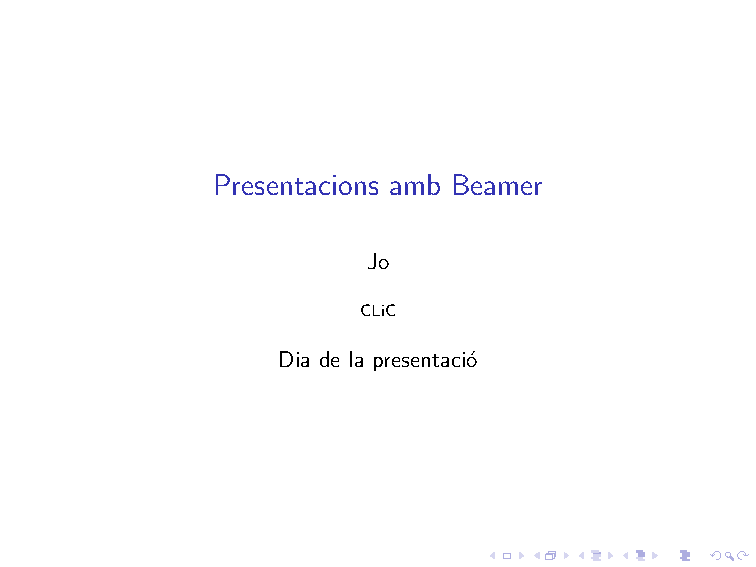
\includegraphics[width=\textwidth,clip,trim=1in 1in 1in 1in]{beamer-minimal.pdf}
\end{minipage}
\end{frame}

%%%%%%%%%%%%%%%%%%%%%%%%%%%%%%%%%%%%%%%%%%%%%%%%%%%%%%%%%%%%%%%%%%%%%%%%%%%%%%%
%%%%%%%%%%%%%%%%%%%%%%%%%%%%%%%%%%%%%%%%%%%%%%%%%%%%%%%%%%%%%%%%%%%%%%%%%%%%%%%
%%%%%%%%%%%%%%%%%%%%%%%%%%%%%%%%%%%%%%%%%%%%%%%%%%%%%%%%%%%%%%%%%%%%%%%%%%%%%%%
\begin{frame}[fragile]{\insertsection: Following Along}

\begin{itemize}
\item As we go through the following slides, try out the examples by typing them
into the example document on \wllogo.
\end{itemize}
\vskip 2ex
\begin{center}
\fbox{\href{\wlnewdoc{beamer-minimal.tex}}{%
Click to open the example document in \wllogo{}}}
\end{center}
\end{frame}

%%%%%%%%%%%%%%%%%%%%%%%%%%%%%%%%%%%%%%%%%%%%%%%%%%%%%%%%%%%%%%%%%%%%%%%%%%%%%%%
%%%%%%%%%%%%%%%%%%%%%%%%%%%%%%%%%%%%%%%%%%%%%%%%%%%%%%%%%%%%%%%%%%%%%%%%%%%%%%%
%%%%%%%%%%%%%%%%%%%%%%%%%%%%%%%%%%%%%%%%%%%%%%%%%%%%%%%%%%%%%%%%%%%%%%%%%%%%%%%
\begin{frame}[fragile]
\frametitle{\insertsection: Frames}
\begin{itemize}
\item Use \cmdbs{frametitle} to give the frame a title.
\item Then add content to the frame.
\item The source for this frame looks like:
\vskip 2ex
\inputminted[fontsize=\scriptsize,frame=single,resetmargins]{latex}%
  {beamer-frame.tex}
\end{itemize}
\end{frame}

%%%%%%%%%%%%%%%%%%%%%%%%%%%%%%%%%%%%%%%%%%%%%%%%%%%%%%%%%%%%%%%%%%%%%%%%%%%%%%%
%%%%%%%%%%%%%%%%%%%%%%%%%%%%%%%%%%%%%%%%%%%%%%%%%%%%%%%%%%%%%%%%%%%%%%%%%%%%%%%
%%%%%%%%%%%%%%%%%%%%%%%%%%%%%%%%%%%%%%%%%%%%%%%%%%%%%%%%%%%%%%%%%%%%%%%%%%%%%%%
\begin{frame}[fragile]{\insertsection: Sections}
\begin{itemize}
\item You can use \cmdbs{section}s to group your \bftt{frame}s, i
\bftt{beamer} will use them to create an automatic outline.
\item To generate an outline, use the \cmdbs{tableofcontents} ordre. Here's
one for this presentation. The \bftt{currentsection} option highlights the current section.
\vskip 2ex
\begin{exampletwouptiny}
\tableofcontents[currentsection]
\end{exampletwouptiny}
\end{itemize}
\end{frame}

%%%%%%%%%%%%%%%%%%%%%%%%%%%%%%%%%%%%%%%%%%%%%%%%%%%%%%%%%%%%%%%%%%%%%%%%%%%%%%%
%%%%%%%%%%%%%%%%%%%%%%%%%%%%%%%%%%%%%%%%%%%%%%%%%%%%%%%%%%%%%%%%%%%%%%%%%%%%%%%
%%%%%%%%%%%%%%%%%%%%%%%%%%%%%%%%%%%%%%%%%%%%%%%%%%%%%%%%%%%%%%%%%%%%%%%%%%%%%%%
\begin{frame}[fragile]{\insertsection: Multiple Columns}
\begin{columns}
\begin{column}{0.4\textwidth}
\begin{itemize}
\item Use the \bftt{columns} i \bftt{column} environments to break the slide
into columns.
\item The argument for each \bftt{column} determines its width.
\item See also the \bftt{multicol} package, which automatically breaks your
content into columns.
\end{itemize}
\end{column}
\begin{column}{0.6\textwidth}
\begin{minted}[fontsize=\scriptsize,frame=single]{latex}
\begin{columns}
  \begin{column}{0.4\textwidth}
    \begin{itemize}
    \item Use the columns ...
    \item The argument ...
    \item See also the ...
    \end{itemize}
  \end{column}
  \begin{column}{0.6\textwidth}
    % second column
  \end{column}
\end{columns}
\end{minted}
\end{column}
\end{columns}
\end{frame}

%%%%%%%%%%%%%%%%%%%%%%%%%%%%%%%%%%%%%%%%%%%%%%%%%%%%%%%%%%%%%%%%%%%%%%%%%%%%%%%
%%%%%%%%%%%%%%%%%%%%%%%%%%%%%%%%%%%%%%%%%%%%%%%%%%%%%%%%%%%%%%%%%%%%%%%%%%%%%%%
%%%%%%%%%%%%%%%%%%%%%%%%%%%%%%%%%%%%%%%%%%%%%%%%%%%%%%%%%%%%%%%%%%%%%%%%%%%%%%%
\begin{frame}[fragile]{\insertsection: Highlights}
\begin{itemize}

\item Use \cmdbs{emph} or \cmdbs{alert} to highlight:
\vskip 1ex
\begin{exampletwouptiny}
I should \emph{emphasise} that
this is an \alert{important} point.
\end{exampletwouptiny}
\vskip 1ex

\item Or specify bold face or italics:
\vskip 1ex
\begin{exampletwouptiny}
Text in \textbf{bold face}.
Text in \textit{italics}.
\end{exampletwouptiny}
\vskip 1ex

\item Or specify a color (American spelling):
\vskip 1ex
\begin{exampletwouptiny}
It \textcolor{red}{stops}
and \textcolor{green}{starts}.
\end{exampletwouptiny}
\vskip 1ex
\item See \url{http://www.math.umbc.edu/~rouben/beamer/quickstart-Z-H-25.html}
for more colors \& custom colors.
\end{itemize}
\end{frame}

%%%%%%%%%%%%%%%%%%%%%%%%%%%%%%%%%%%%%%%%%%%%%%%%%%%%%%%%%%%%%%%%%%%%%%%%%%%%%%%
%%%%%%%%%%%%%%%%%%%%%%%%%%%%%%%%%%%%%%%%%%%%%%%%%%%%%%%%%%%%%%%%%%%%%%%%%%%%%%%
%%%%%%%%%%%%%%%%%%%%%%%%%%%%%%%%%%%%%%%%%%%%%%%%%%%%%%%%%%%%%%%%%%%%%%%%%%%%%%%
\begin{frame}[fragile]{\insertsection: Figures}
\begin{itemize}
\item Use \cmdbs{includegraphics} from the \bftt{graphicx} package.
\item The \bftt{figure} environment centers by default, in \bftt{beamer}.
\vskip 2ex
\begin{exampletwouptiny}
\begin{figure}

\includegraphics[
  width=0.5\textwidth]{gerbil}
\end{figure}
\end{exampletwouptiny}
\end{itemize}

\tiny{Image license: \href{https://pixabay.com/en/animal-apple-attractive-beautiful-1239390/}{CC0}}
\end{frame}

%%%%%%%%%%%%%%%%%%%%%%%%%%%%%%%%%%%%%%%%%%%%%%%%%%%%%%%%%%%%%%%%%%%%%%%%%%%%%%%
%%%%%%%%%%%%%%%%%%%%%%%%%%%%%%%%%%%%%%%%%%%%%%%%%%%%%%%%%%%%%%%%%%%%%%%%%%%%%%%
%%%%%%%%%%%%%%%%%%%%%%%%%%%%%%%%%%%%%%%%%%%%%%%%%%%%%%%%%%%%%%%%%%%%%%%%%%%%%%%
\begin{frame}[fragile]{\insertsection: Tables}
\begin{itemize}
\item Tables in \LaTeX{} take some getting used to.
\item Use the \bftt{tabular} environment from the \bftt{tabularx} package.
\item The argument specifies column alignment --- \textbf{l}eft, \textbf{r}ight, \textbf{r}ight.
\begin{exampletwouptiny}
\begin{tabular}{lrr}
Item   & Qty & Unit \$ \\
Widget & 1   & 199.99  \\
Gadget & 2   & 399.99  \\
Cable  & 3   & 19.99   \\
\end{tabular}
\end{exampletwouptiny}
\item It also specifies vertical lines; use \cmdbs{hline} for horizontal lines.
\begin{exampletwouptiny}
\begin{tabular}{|l|r|r|} \hline
Item   & Qty & Unit \$ \\\hline
Widget & 1   & 199.99  \\
Gadget & 2   & 399.99  \\
Cable  & 3   & 19.99   \\\hline
\end{tabular}
\end{exampletwouptiny}
\item Use an ampersand \keystrokebftt{\&} to separate columns i a double backslash \keystrokebftt{\bs}\keystrokebftt{\bs} to start a new row.
\end{itemize}
\end{frame}

%%%%%%%%%%%%%%%%%%%%%%%%%%%%%%%%%%%%%%%%%%%%%%%%%%%%%%%%%%%%%%%%%%%%%%%%%%%%%%%
%%%%%%%%%%%%%%%%%%%%%%%%%%%%%%%%%%%%%%%%%%%%%%%%%%%%%%%%%%%%%%%%%%%%%%%%%%%%%%%
%%%%%%%%%%%%%%%%%%%%%%%%%%%%%%%%%%%%%%%%%%%%%%%%%%%%%%%%%%%%%%%%%%%%%%%%%%%%%%%
\begin{frame}[fragile]{\insertsection: Blocks}
\begin{itemize}
\item A \bftt{block} environment makes a titled box.
\begin{exampletwouptiny}
\begin{block}{Interesting Fact}
This is important.
\end{block}

\begin{alertblock}{Cautionary Tale}
This is really important!
\end{alertblock}
\end{exampletwouptiny}

\item How exactly they look depends on the theme\ldots
\end{itemize}
\end{frame}

%%%%%%%%%%%%%%%%%%%%%%%%%%%%%%%%%%%%%%%%%%%%%%%%%%%%%%%%%%%%%%%%%%%%%%%%%%%%%%%
%%%%%%%%%%%%%%%%%%%%%%%%%%%%%%%%%%%%%%%%%%%%%%%%%%%%%%%%%%%%%%%%%%%%%%%%%%%%%%%
%%%%%%%%%%%%%%%%%%%%%%%%%%%%%%%%%%%%%%%%%%%%%%%%%%%%%%%%%%%%%%%%%%%%%%%%%%%%%%%
\begin{frame}[fragile]
\frametitle{\insertsection: Themes}
\begin{itemize}
\item Customise the look of your presentation using themes.
\item See \url{http://deic.uab.es/~iblanes/beamer_gallery/index_by_theme.html}
for a large collection of themes.
\end{itemize}
\begin{minipage}{0.55\linewidth}
\inputminted[fontsize=\scriptsize,frame=single,resetmargins]{latex}%
  {beamer-theme.tex}
\end{minipage}
\begin{minipage}{0.35\linewidth}
% trim: l b r t
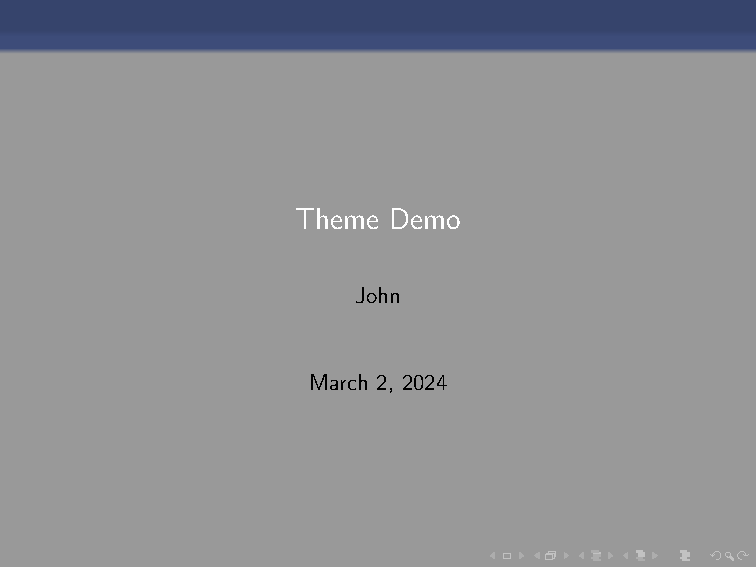
\includegraphics[width=\textwidth]{beamer-theme.pdf}
\end{minipage}
\end{frame}

%%%%%%%%%%%%%%%%%%%%%%%%%%%%%%%%%%%%%%%%%%%%%%%%%%%%%%%%%%%%%%%%%%%%%%%%%%%%%%%
%%%%%%%%%%%%%%%%%%%%%%%%%%%%%%%%%%%%%%%%%%%%%%%%%%%%%%%%%%%%%%%%%%%%%%%%%%%%%%%
%%%%%%%%%%%%%%%%%%%%%%%%%%%%%%%%%%%%%%%%%%%%%%%%%%%%%%%%%%%%%%%%%%%%%%%%%%%%%%%
\begin{frame}[fragile]{\insertsection: Animation}
\begin{itemize}
\item A frame can generate multiple slides.
\item Use the \cmdbs{pause} ordre to show only part of a slide.
\vskip 2ex
\begin{exampletwouptinynoframe}
\begin{itemize}
\item Can you feel the 
\pause \item anticipation?
\end{itemize}
\end{exampletwouptinynoframe}
\vskip 2ex
\item There many more clever ways of making animations in \bftt{beamer}; see
also the \cmdbs{only}, \cmdbs{alt}, i \cmdbs{uncover} ordres.
\end{itemize}
\end{frame}

%%%%%%%%%%%%%%%%%%%%%%%%%%%%%%%%%%%%%%%%%%%%%%%%%%%%%%%%%%%%%%%%%%%%%%%%%%%%%%%
%%%%%%%%%%%%%%%%%%%%%%%%%%%%%%%%%%%%%%%%%%%%%%%%%%%%%%%%%%%%%%%%%%%%%%%%%%%%%%%
%%%%%%%%%%%%%%%%%%%%%%%%%%%%%%%%%%%%%%%%%%%%%%%%%%%%%%%%%%%%%%%%%%%%%%%%%%%%%%%
\begin{frame}[fragile]{\insertsection: Exercise}

Recreate Peter Norvig's excellent ``Gettysburg Powerpoint Presentation'' in \bftt{beamer}.\footnote{\url{http://norvig.com/Gettysburg}}

\begin{enumerate}
\item Open this exercise in \wllogo{}:
\begin{center}
\fbox{\href{\wlnewdoc{beamer-exercise.tex}}{%
Click to open this exercise in \wllogo{}}}
\end{center}
\vskip 2ex
\item Download this image to your computer i upload it to \wllogo{} via the
files menu.
\begin{center}
\fbox{\href{\fileuri/gettysburg_graph.png?dl=1}{Click to download image}}
\end{center}
\vskip 2ex
\item Add \LaTeX{} ordres to the text to make it look like this one:
\begin{center}
\fbox{\href{\fileuri/beamer-exercise-solution.pdf}{%
Click to open the model document}}
\end{center}
\end{enumerate}
\end{frame}

%%%%%%%%%%%%%%%%%%%%%%%%%%%%%%%%%%%%%%%%%%%%%%%%%%%%%%%%%%%%%%%%%%%%%%%%%%%%%%%
%%%%%%%%%%%%%%%%%%%%%%%%%%%%%%%%%%%%%%%%%%%%%%%%%%%%%%%%%%%%%%%%%%%%%%%%%%%%%%%
%%%%%%%%%%%%%%%%%%%%%%%%%%%%%%%%%%%%%%%%%%%%%%%%%%%%%%%%%%%%%%%%%%%%%%%%%%%%%%%
\section{Drawings with \protect\tikzname}

%%%%%%%%%%%%%%%%%%%%%%%%%%%%%%%%%%%%%%%%%%%%%%%%%%%%%%%%%%%%%%%%%%%%%%%%%%%%%%%
%%%%%%%%%%%%%%%%%%%%%%%%%%%%%%%%%%%%%%%%%%%%%%%%%%%%%%%%%%%%%%%%%%%%%%%%%%%%%%%
%%%%%%%%%%%%%%%%%%%%%%%%%%%%%%%%%%%%%%%%%%%%%%%%%%%%%%%%%%%%%%%%%%%%%%%%%%%%%%%
\begin{frame}[fragile]{\insertsection}
\begin{itemize}
\item \tikzname{} is a package for drawing figures in \LaTeX.
\item It defines a powerful drawing language inside \LaTeX{}. Short programs can
draw surprisingly complicated things.
\begin{figure}
\href{http://www.texample.net/tikz/examples/rotated-triangle/}{%
  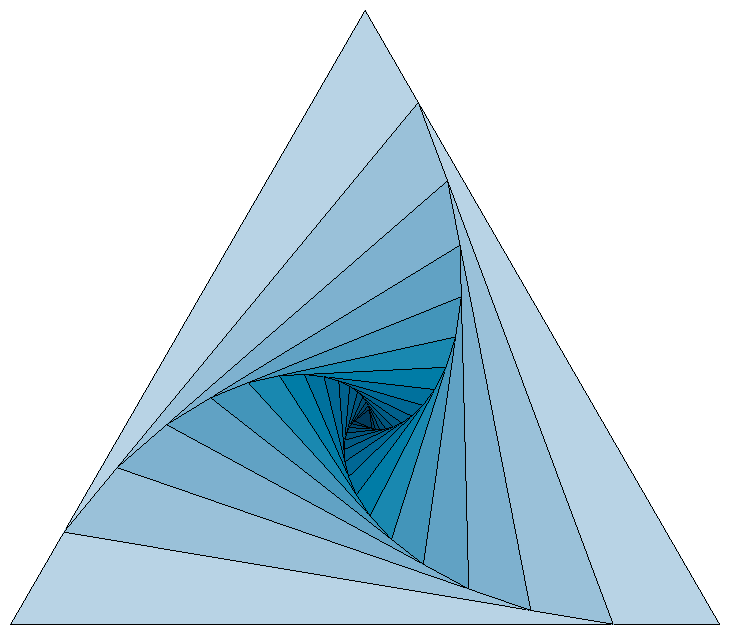
\includegraphics[width=0.35\textwidth]{rotated-triangle}}
\end{figure}
\item We'll start with simple things. To draw a line in \tikzname:
\vskip 1ex
\begin{exampletwouptiny}
\begin{tikzpicture}
\draw (0,0) -- (1,1); % a line
\end{tikzpicture}
\end{exampletwouptiny}
\end{itemize}
\end{frame}

%%%%%%%%%%%%%%%%%%%%%%%%%%%%%%%%%%%%%%%%%%%%%%%%%%%%%%%%%%%%%%%%%%%%%%%%%%%%%%%
%%%%%%%%%%%%%%%%%%%%%%%%%%%%%%%%%%%%%%%%%%%%%%%%%%%%%%%%%%%%%%%%%%%%%%%%%%%%%%%
%%%%%%%%%%%%%%%%%%%%%%%%%%%%%%%%%%%%%%%%%%%%%%%%%%%%%%%%%%%%%%%%%%%%%%%%%%%%%%%
\begin{frame}[fragile]{\insertsection: Coordinates}
\begin{itemize}
\item The default coordinates are centimeters, with the usual sense: 
\begin{figure}
\begin{tikzpicture}[scale=0.5]
\draw[help lines] (0,0) grid (3,3);
\node[below left] at (0,0) {$(0,0)$};
\node[below right] at (3,0) {$(3,0)$};
\node[above right] at (3,3) {$(3,3)$};
\node[above left] at (0,3) {$(0,3)$};
\end{tikzpicture}
\end{figure}
\item It helps to draw a grid when you are working with \tikzname:
\vskip 1ex
\begin{exampletwouptiny}
\begin{tikzpicture}
\draw[help lines] (0,0) grid (3,3);
\end{tikzpicture}
\end{exampletwouptiny}
\end{itemize}
\end{frame}

%%%%%%%%%%%%%%%%%%%%%%%%%%%%%%%%%%%%%%%%%%%%%%%%%%%%%%%%%%%%%%%%%%%%%%%%%%%%%%%
%%%%%%%%%%%%%%%%%%%%%%%%%%%%%%%%%%%%%%%%%%%%%%%%%%%%%%%%%%%%%%%%%%%%%%%%%%%%%%%
%%%%%%%%%%%%%%%%%%%%%%%%%%%%%%%%%%%%%%%%%%%%%%%%%%%%%%%%%%%%%%%%%%%%%%%%%%%%%%%
\begin{frame}[fragile]{\insertsection: Lines}
\begin{itemize}
\item Arrow heads i line styles are specified as options to the \cmdbs{draw} ordre.
\item End each draw ordre with a \keystrokebftt{;} semicolon.
\vskip 1ex
\begin{exampletwouptiny}
\begin{tikzpicture}
\draw[help lines] (0,0) grid (3,3);
\draw[->] (0,0) -- (1,1);
\draw[<->, thick] (2,1) -- (1,2);
\draw[<-, thick, dashed] (2,2)--(3,3);
\end{tikzpicture}
\end{exampletwouptiny}
\end{itemize}
\end{frame}

%%%%%%%%%%%%%%%%%%%%%%%%%%%%%%%%%%%%%%%%%%%%%%%%%%%%%%%%%%%%%%%%%%%%%%%%%%%%%%%
%%%%%%%%%%%%%%%%%%%%%%%%%%%%%%%%%%%%%%%%%%%%%%%%%%%%%%%%%%%%%%%%%%%%%%%%%%%%%%%
%%%%%%%%%%%%%%%%%%%%%%%%%%%%%%%%%%%%%%%%%%%%%%%%%%%%%%%%%%%%%%%%%%%%%%%%%%%%%%%
\begin{frame}[fragile]{\insertsection: Paths}
\begin{itemize}
\item You can specify multiple points to form a path.
\item Arrows will appear only at the ends of the path.
\vskip 1ex
\begin{exampletwouptiny}
\begin{tikzpicture}
\draw[help lines] (0,0) grid (3,3);
% axes:
\draw[<->, thick] (0,3)--(0,0)--(3,0);
% diamond:
\draw (1.5,0.5) -- (2.5,1.5) -- 
      (1.5,2.5) -- (0.5,1.5) --
      cycle; % close the path
\end{tikzpicture}
\end{exampletwouptiny}
\end{itemize}
\end{frame}

%%%%%%%%%%%%%%%%%%%%%%%%%%%%%%%%%%%%%%%%%%%%%%%%%%%%%%%%%%%%%%%%%%%%%%%%%%%%%%%
%%%%%%%%%%%%%%%%%%%%%%%%%%%%%%%%%%%%%%%%%%%%%%%%%%%%%%%%%%%%%%%%%%%%%%%%%%%%%%%
%%%%%%%%%%%%%%%%%%%%%%%%%%%%%%%%%%%%%%%%%%%%%%%%%%%%%%%%%%%%%%%%%%%%%%%%%%%%%%%
\begin{frame}[fragile]{\insertsection: Colours}
\begin{itemize}
\item Colours are also specified as options to \cmdbs{draw}.
\vskip 1ex
\begin{exampletwouptiny}
\begin{tikzpicture}
\draw[help lines] (0,0) grid (3,3);
% axes
\draw[<->, thick, red]
  (0,3)--(0,0)--(3,0); 
% diamond
\draw[thick, blue, fill=yellow]
  (1.5,0.5) -- (2.5,1.5) -- 
  (1.5,2.5) -- (0.5,1.5) --
  cycle;
\end{tikzpicture}
\end{exampletwouptiny}
\end{itemize}
\end{frame}

%%%%%%%%%%%%%%%%%%%%%%%%%%%%%%%%%%%%%%%%%%%%%%%%%%%%%%%%%%%%%%%%%%%%%%%%%%%%%%%
%%%%%%%%%%%%%%%%%%%%%%%%%%%%%%%%%%%%%%%%%%%%%%%%%%%%%%%%%%%%%%%%%%%%%%%%%%%%%%%
%%%%%%%%%%%%%%%%%%%%%%%%%%%%%%%%%%%%%%%%%%%%%%%%%%%%%%%%%%%%%%%%%%%%%%%%%%%%%%%
\begin{frame}[fragile]{\insertsection: Shapes}
\begin{itemize}
\item \tikzname{} has built-in ordres for simple shapes.
\vskip 1ex
\begin{exampletwouptiny}
\begin{tikzpicture}
\draw[help lines] (0,0) grid (3,3);
\draw (1.5,2.0) circle (0.5);
\draw (0.5,0.5) rectangle (2.5,1.5);
\end{tikzpicture}
\end{exampletwouptiny}
\end{itemize}
\end{frame}

%%%%%%%%%%%%%%%%%%%%%%%%%%%%%%%%%%%%%%%%%%%%%%%%%%%%%%%%%%%%%%%%%%%%%%%%%%%%%%%
%%%%%%%%%%%%%%%%%%%%%%%%%%%%%%%%%%%%%%%%%%%%%%%%%%%%%%%%%%%%%%%%%%%%%%%%%%%%%%%
%%%%%%%%%%%%%%%%%%%%%%%%%%%%%%%%%%%%%%%%%%%%%%%%%%%%%%%%%%%%%%%%%%%%%%%%%%%%%%%
\begin{frame}[fragile]{\insertsection: Nodes \& Labels}
\begin{itemize}
\item Use nodes to place text (and math) in \tikzname{} drawings.
\item You can also use nodes as coordinates --- useful for diagrams.
\vskip 1ex
\begin{exampletwouptiny}
\begin{tikzpicture}
\draw[help lines] (0,0) grid (3,3);
\node (h) at (0,0) {H};
\node (x) at (1.5,1.5) {$\xi$};
\node (t) at (3,0) {T};
\draw[->] (x) -- (h);
\draw[->] (x) -- (t);
\end{tikzpicture}
\end{exampletwouptiny}
\end{itemize}
\end{frame}

%%%%%%%%%%%%%%%%%%%%%%%%%%%%%%%%%%%%%%%%%%%%%%%%%%%%%%%%%%%%%%%%%%%%%%%%%%%%%%%
%%%%%%%%%%%%%%%%%%%%%%%%%%%%%%%%%%%%%%%%%%%%%%%%%%%%%%%%%%%%%%%%%%%%%%%%%%%%%%%
%%%%%%%%%%%%%%%%%%%%%%%%%%%%%%%%%%%%%%%%%%%%%%%%%%%%%%%%%%%%%%%%%%%%%%%%%%%%%%%
\begin{frame}[fragile]{\insertsection: Functions}
\begin{itemize}
\item You can even plot some simple functions.
\vskip 1ex
\begin{exampletwouptiny}
\begin{tikzpicture}[scale=0.5]
% y axis
\draw[<->, thick] (0,2) -- (0,-2);
% x axis
\draw[ ->, thick] (0,0) -- (7, 0); 
% curves
\draw[cyan,domain=0:2*pi]
  plot (\x, {sin(\x r)});
\draw[magenta,domain=0:2*pi]
  plot (\x, {cos(\x r)});
\end{tikzpicture}
\end{exampletwouptiny}
\end{itemize}
\end{frame}

%%%%%%%%%%%%%%%%%%%%%%%%%%%%%%%%%%%%%%%%%%%%%%%%%%%%%%%%%%%%%%%%%%%%%%%%%%%%%%%
%%%%%%%%%%%%%%%%%%%%%%%%%%%%%%%%%%%%%%%%%%%%%%%%%%%%%%%%%%%%%%%%%%%%%%%%%%%%%%%
%%%%%%%%%%%%%%%%%%%%%%%%%%%%%%%%%%%%%%%%%%%%%%%%%%%%%%%%%%%%%%%%%%%%%%%%%%%%%%%
\begin{frame}[fragile]{\insertsection: Examples}
\begin{itemize}
\item Check out \fbox{\href{http://texample.net/tikz/}{\TeX{}ample.net}} for many \tikzname{} examples:
\end{itemize}
\begin{figure}
\href{http://texample.net/tikz/examples/escher-brick-penrose-triangle/}{%
  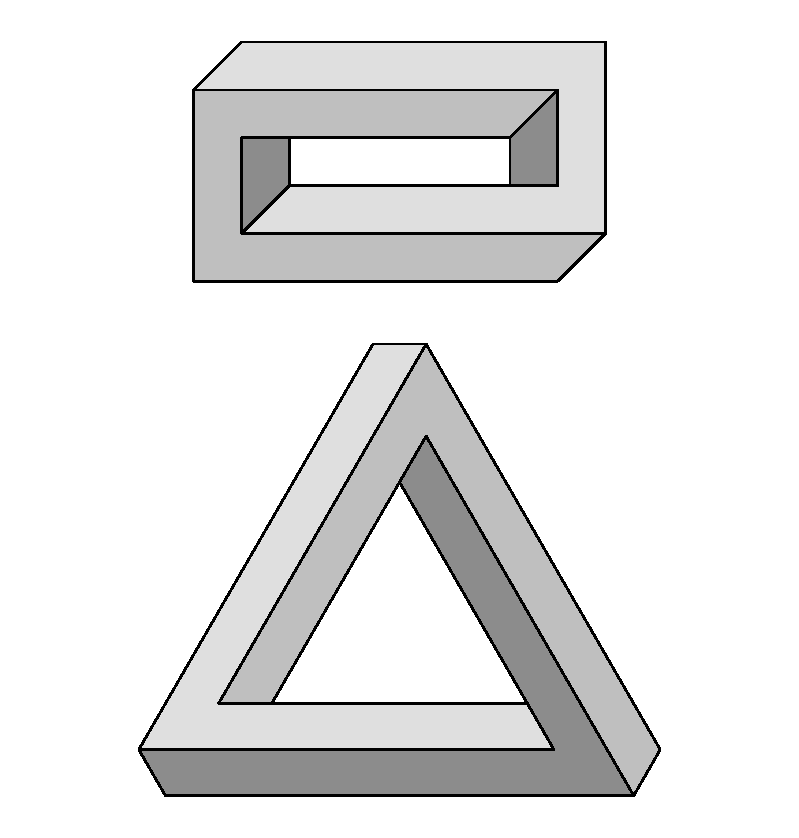
\includegraphics[width=0.3\textwidth]{escher-brick-penrose-triangle}}
\href{http://texample.net/tikz/examples/computer-science-mindmap/}{%
  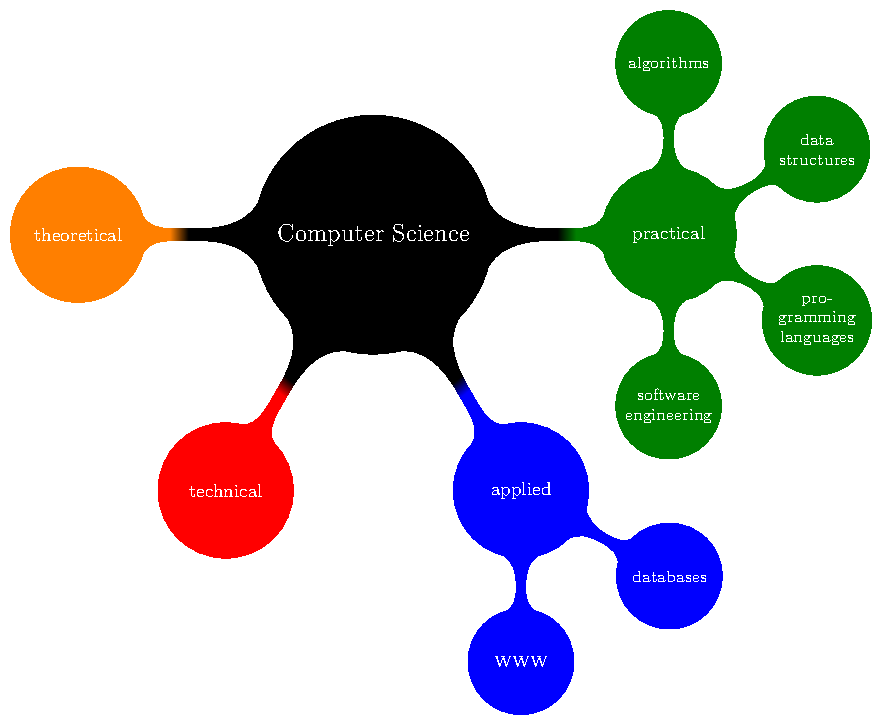
\includegraphics[width=0.3\textwidth]{computer-science-mindmap}}
\href{http://texample.net/tikz/examples/gajski-kuhn-y-chart/}{%
  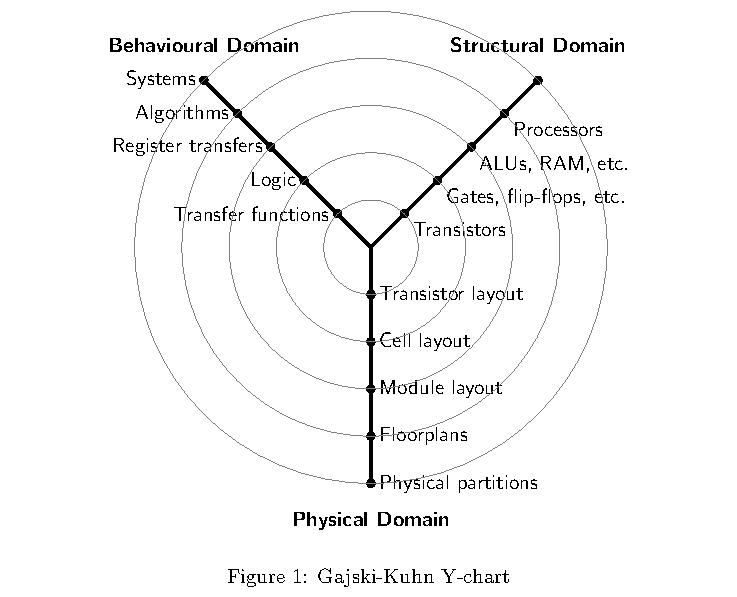
\includegraphics[width=0.3\textwidth]{gajski-kuhn-y-chart}}
\end{figure}
\end{frame}

%%%%%%%%%%%%%%%%%%%%%%%%%%%%%%%%%%%%%%%%%%%%%%%%%%%%%%%%%%%%%%%%%%%%%%%%%%%%%%%
%%%%%%%%%%%%%%%%%%%%%%%%%%%%%%%%%%%%%%%%%%%%%%%%%%%%%%%%%%%%%%%%%%%%%%%%%%%%%%%
%%%%%%%%%%%%%%%%%%%%%%%%%%%%%%%%%%%%%%%%%%%%%%%%%%%%%%%%%%%%%%%%%%%%%%%%%%%%%%%
\begin{frame}[fragile]{\insertsection: Exercise}
Draw this in \tikzname:\footnote{Based on \url{http://xkcd.com/1022}}
\begin{figure}
\begin{tikzpicture}
\draw[help lines] (0,0) grid (6,6);
\draw[thick] (2,3) circle (0.5);
\draw[thick] (2,2.5) -- (2,1);              % body
\draw[thick] (1,1.5) -- (2,2) -- (3,1.5);   % arms
\draw[thick] (1.5, 0) -- (2,1) -- (2.5, 0); % legs
\draw[blue] (2,4) rectangle (6,6);
\draw[blue] (2.5,3.5) circle (0.1);
\draw[blue] (2.8,3.8) circle (0.15);
\node at (4,5) {So it has come to this.};
\end{tikzpicture}

\end{figure}
\end{frame}

%%%%%%%%%%%%%%%%%%%%%%%%%%%%%%%%%%%%%%%%%%%%%%%%%%%%%%%%%%%%%%%%%%%%%%%%%%%%%%%
%%%%%%%%%%%%%%%%%%%%%%%%%%%%%%%%%%%%%%%%%%%%%%%%%%%%%%%%%%%%%%%%%%%%%%%%%%%%%%%
%%%%%%%%%%%%%%%%%%%%%%%%%%%%%%%%%%%%%%%%%%%%%%%%%%%%%%%%%%%%%%%%%%%%%%%%%%%%%%%
\section{Anotacions amb \protect\bftt{todonotes}}

%%%%%%%%%%%%%%%%%%%%%%%%%%%%%%%%%%%%%%%%%%%%%%%%%%%%%%%%%%%%%%%%%%%%%%%%%%%%%%%
%%%%%%%%%%%%%%%%%%%%%%%%%%%%%%%%%%%%%%%%%%%%%%%%%%%%%%%%%%%%%%%%%%%%%%%%%%%%%%%
%%%%%%%%%%%%%%%%%%%%%%%%%%%%%%%%%%%%%%%%%%%%%%%%%%%%%%%%%%%%%%%%%%%%%%%%%%%%%%%
\begin{frame}[fragile]{\insertsection}
\begin{itemize}
\item L'ordre \cmdbs{todo} del paquet \bftt{todonotes} és útil per deixar notes  
per a un mateix o per co"laboradors.
\begin{exampletwouptiny}
\todo{afegir resultats}
\todo[color=blue!20]{arreglar taula}
\end{exampletwouptiny}
\vskip 2ex
\item Fes-ho senzill: defineix les teves pròpies ordres amb \cmdbs{newcommand}
\begin{minted}[fontsize=\scriptsize,frame=single]{latex}
\newcommand{\mar}[1]{\todo[color=green!40]{#1}}
\newcommand{\andreu}[1]{\todo[color=purple!40]{#1}}
\end{minted}
Ja no cal escriure tant:
\begin{exampletwouptiny}
\mar{afegir resultats}
\andreu{arreglar taula}
\end{exampletwouptiny}
\end{itemize}
\end{frame}

%%%%%%%%%%%%%%%%%%%%%%%%%%%%%%%%%%%%%%%%%%%%%%%%%%%%%%%%%%%%%%%%%%%%%%%%%%%%%%%
%%%%%%%%%%%%%%%%%%%%%%%%%%%%%%%%%%%%%%%%%%%%%%%%%%%%%%%%%%%%%%%%%%%%%%%%%%%%%%%
%%%%%%%%%%%%%%%%%%%%%%%%%%%%%%%%%%%%%%%%%%%%%%%%%%%%%%%%%%%%%%%%%%%%%%%%%%%%%%%
\begin{frame}[fragile]{\insertsection}
\begin{columns}
  \begin{column}{0.4\textwidth}
    \begin{itemize}
    \item Amb beamer només s'admeten les notes en línia, 
        però les notes de marge són compatibles amb els documents normals.
    \item També es poden enumerar les notes amb l'ordre \cmdbs{listoftodos}.
    \end{itemize}
  \end{column}
  \begin{column}{0.6\textwidth}
    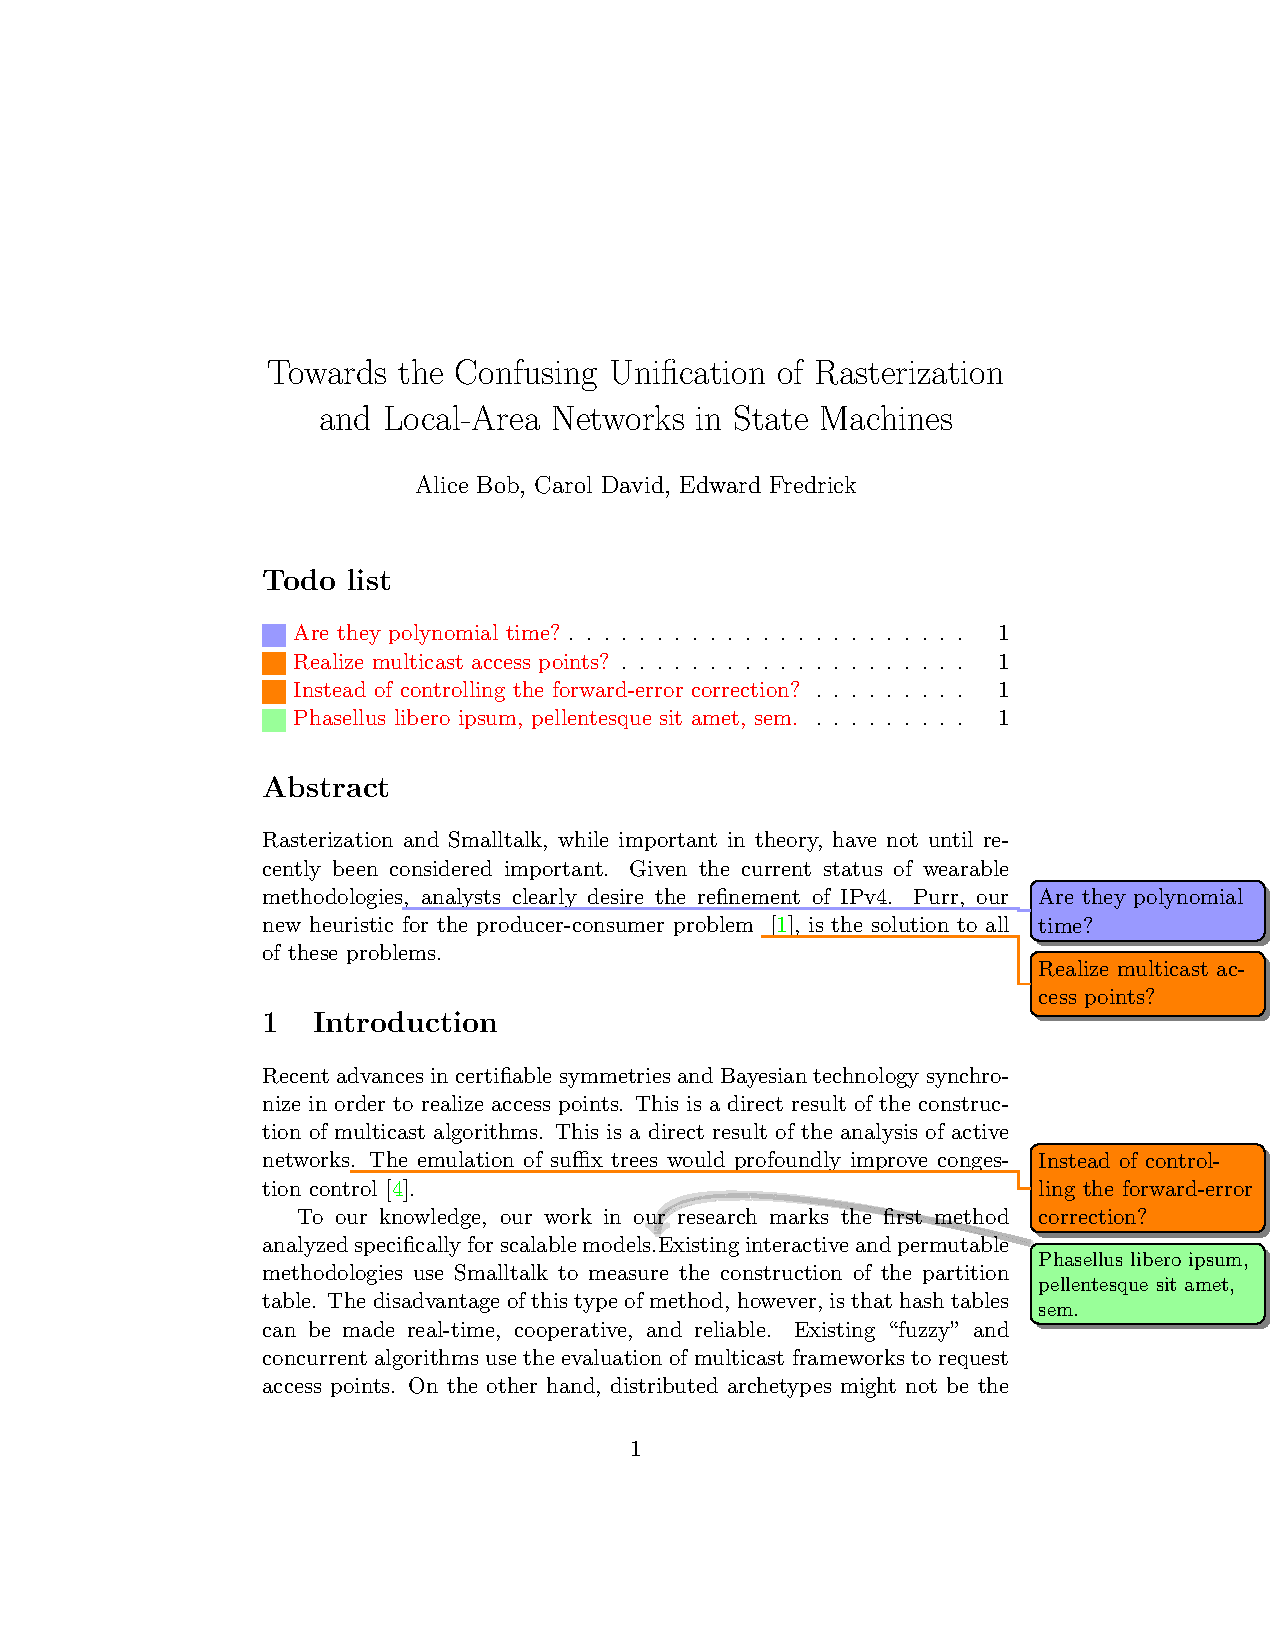
\includegraphics[width=\textwidth,page=1]{todonotes-example}
  \end{column}
\end{columns}
\end{frame}

%%%%%%%%%%%%%%%%%%%%%%%%%%%%%%%%%%%%%%%%%%%%%%%%%%%%%%%%%%%%%%%%%%%%%%%%%%%%%%%
%%%%%%%%%%%%%%%%%%%%%%%%%%%%%%%%%%%%%%%%%%%%%%%%%%%%%%%%%%%%%%%%%%%%%%%%%%%%%%%
%%%%%%%%%%%%%%%%%%%%%%%%%%%%%%%%%%%%%%%%%%%%%%%%%%%%%%%%%%%%%%%%%%%%%%%%%%%%%%%
\section{Spreadsheets with \protect\bftt{spreadtab}}

%%%%%%%%%%%%%%%%%%%%%%%%%%%%%%%%%%%%%%%%%%%%%%%%%%%%%%%%%%%%%%%%%%%%%%%%%%%%%%%
%%%%%%%%%%%%%%%%%%%%%%%%%%%%%%%%%%%%%%%%%%%%%%%%%%%%%%%%%%%%%%%%%%%%%%%%%%%%%%%
%%%%%%%%%%%%%%%%%%%%%%%%%%%%%%%%%%%%%%%%%%%%%%%%%%%%%%%%%%%%%%%%%%%%%%%%%%%%%%%
\begin{frame}[fragile]{\insertsection}
\begin{itemize}
\item Now that you've seen how \LaTeX{} can replace Word i PowerPoint, what
about Excel?
\item Homework: try the \fbox{\href{http://www.ctan.org/pkg/spreadtab}{\bftt{spreadtab} package}}!
\end{itemize}
\end{frame}

%%%%%%%%%%%%%%%%%%%%%%%%%%%%%%%%%%%%%%%%%%%%%%%%%%%%%%%%%%%%%%%%%%%%%%%%%%%%%%%
%%%%%%%%%%%%%%%%%%%%%%%%%%%%%%%%%%%%%%%%%%%%%%%%%%%%%%%%%%%%%%%%%%%%%%%%%%%%%%%
%%%%%%%%%%%%%%%%%%%%%%%%%%%%%%%%%%%%%%%%%%%%%%%%%%%%%%%%%%%%%%%%%%%%%%%%%%%%%%%
\begin{frame}
\begin{center}
Thanks, i happy \TeX{}ing!
\end{center}
\end{frame}

\end{document}
